\documentclass[10pt,twocolumn]{article}

\usepackage[utf8]{inputenc}
\usepackage[spanish]{babel}
\usepackage[margin=2cm]{geometry}
\usepackage{graphicx}
\usepackage{amsmath,amssymb,amsthm}
\usepackage{booktabs}
\usepackage{caption}
\usepackage{subcaption}
\usepackage{hyperref}
\usepackage{xcolor}
\usepackage{enumitem}
\usepackage{float}

\definecolor{accentblue}{HTML}{6366F1}
\definecolor{accentgreen}{HTML}{10B981}

\newtheorem{definition}{Definición}
\newtheorem{proposition}{Proposición}
\newtheorem{theorem}{Teorema}

\title{\textbf{Reporte del Experimento 3:}\\Ablación Completa 3$\times$3 sobre Dataset Sintético de Alta Dificultad Topológica}
\author{Pontificia Universidad Javeriana\\Maestría en Ingeniería}
\date{Abril 2026}

\begin{document}
\maketitle

\begin{abstract}
Se presenta una comparación sistemática de tres arquitecturas de segmentación (BaselineUNet, InputFusionTDASegUNet, BottleneckFusionTDASegUNet) combinadas con tres funciones de pérdida (dice, betti, dice+betti) sobre un dataset sintético topológicamente desafiante. Los resultados muestran que la pérdida de Betti Matching reduce los errores topológicos $\beta_1$ en un 75--100\% sin sacrificar el Dice, y que nuestra arquitectura propuesta (BottleneckFusion) alcanza \textbf{cero errores $\beta_1$} cuando se combina con supervisión topológica, superando la implementación paper-faithful (InputFusion). Se propone el \emph{Principio de Separación de Gradientes} como explicación arquitectónica.
\end{abstract}

% ============================================================
\section{Objetivo}

Determinar si (a) la información topológica como entrada mejora la segmentación, (b) la pérdida topológica reduce errores topológicos, y (c) la arquitectura de doble encoder propuesta amplifica el efecto de la supervisión topológica.

% ============================================================
\section{Descripción Matemática de las Arquitecturas}

\subsection{Preliminares: U-Net}

Una U-Net de profundidad $L$ es una función $f_\theta: \mathbb{R}^{C_0 \times H \times W} \to [0,1]^{1 \times H \times W}$ definida por:
\begin{equation}
f_\theta = \sigma_{\text{out}} \circ \text{Conv}_{1\times1} \circ D_1 \circ \cdots \circ D_L \circ B \circ E_L \circ \cdots \circ E_1
\end{equation}
donde $E_\ell$ son bloques encoder, $B$ es el bottleneck, $D_\ell$ son bloques decoder con skip connections $s_\ell = E_\ell(\cdot)$, y $\sigma_{\text{out}}$ es la sigmoide.

\begin{definition}[Bloque Encoder]
Un bloque encoder al nivel $\ell$ es la composición:
\begin{equation}
E_\ell = \text{Pool} \circ \sigma \circ \text{BN} \circ \text{Conv}_2 \circ \sigma \circ \text{BN} \circ \text{Conv}_1
\end{equation}
donde $\sigma$ es ReLU, BN es batch normalization, $\text{Conv}_i$ son convoluciones $3\times3$, y Pool es max pooling $2\times2$.
\end{definition}

\subsection{BaselineUNet (Referencia)}

\begin{equation}
f_{\text{Baseline}}(I) = \text{UNet}(I), \quad I \in \mathbb{R}^{1 \times 128 \times 128}
\end{equation}

U-Net estándar con 1 canal de entrada. Ignora las características TDA. \textbf{1,926,433 parámetros.}

\subsection{InputFusionTDASegUNet (Paper)}

\begin{equation}
f_{\text{Input}}(I, \tau) = \text{UNet}(\text{Cat}(I, \text{PI}_0, \text{PI}_1))
\end{equation}

donde $\text{Cat}: \mathbb{R}^{1 \times H \times W} \times \mathbb{R}^{2 \times H \times W} \to \mathbb{R}^{3 \times H \times W}$ es la concatenación por canales. Un \textbf{mismo encoder} procesa las 3 modalidades. La primera convolución tiene kernel $W \in \mathbb{R}^{32 \times 3 \times 3 \times 3}$: los gradientes de \emph{todas} las pérdidas pasan por los \emph{mismos} pesos. \textbf{1,927,009 parámetros.}

\begin{figure}[H]
\centering
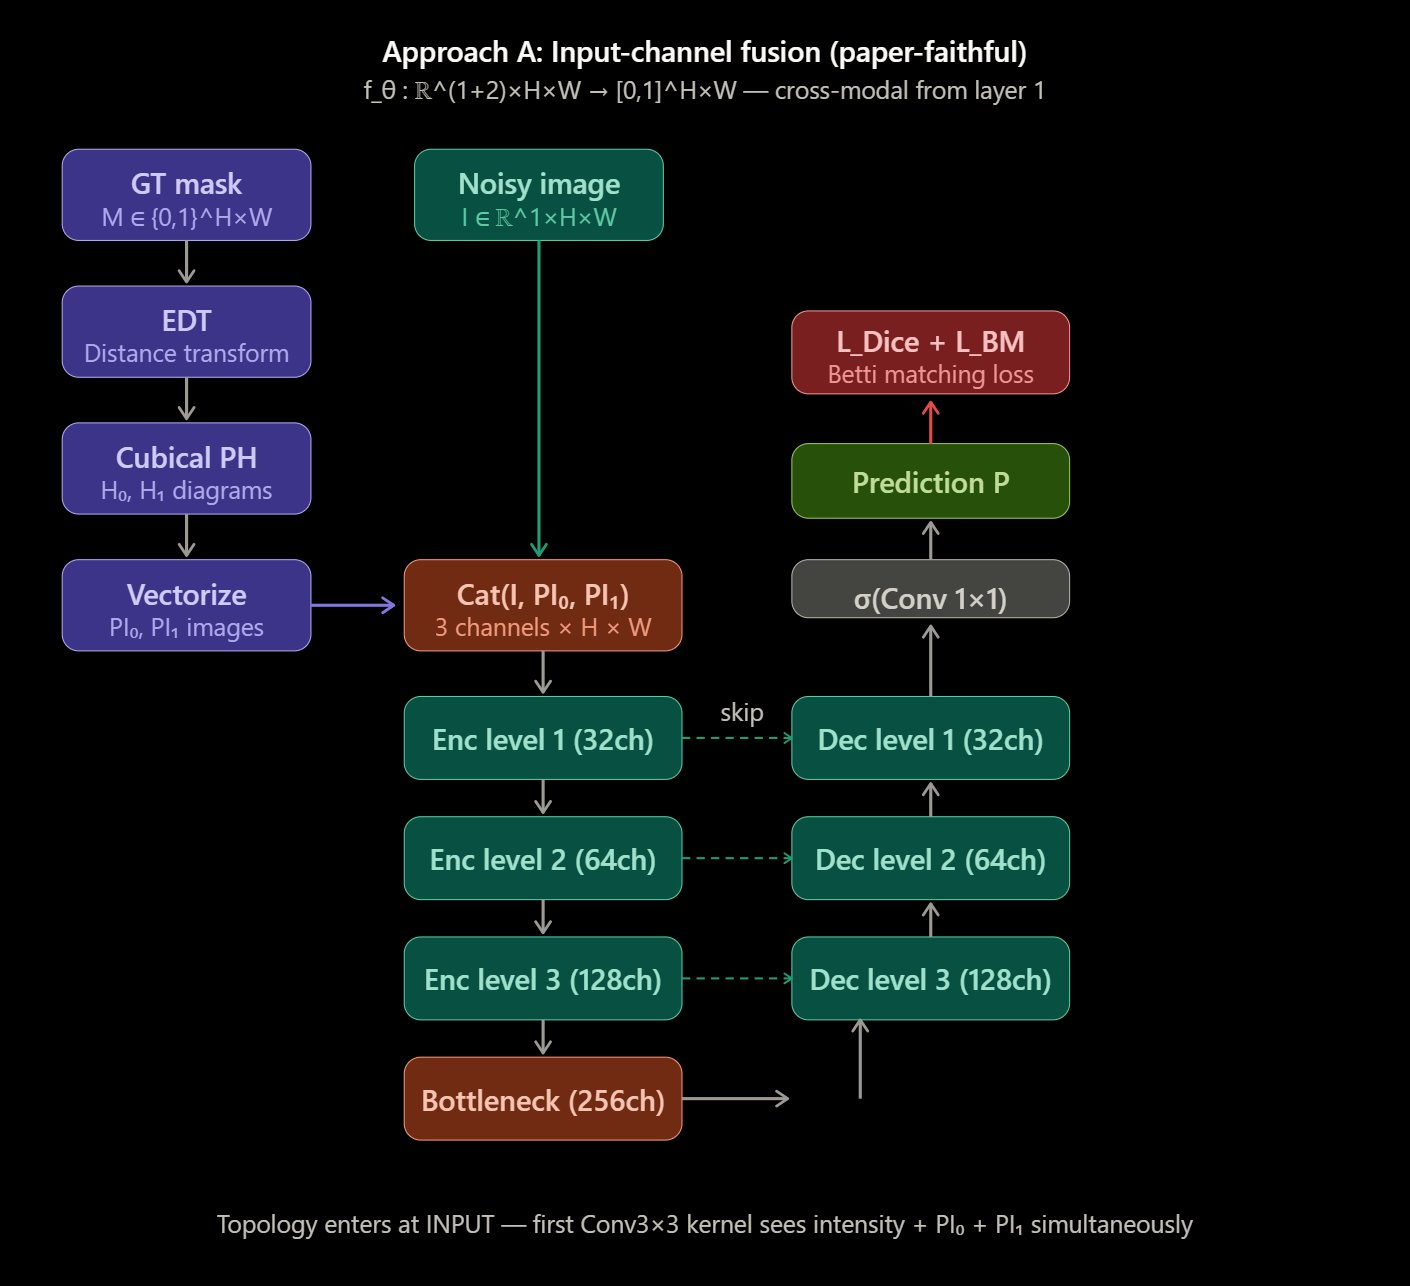
\includegraphics[width=\columnwidth]{arch_inputfusion.png}
\caption{InputFusion: concatenación de imagen + PI$_0$ + PI$_1$ como 3 canales de entrada a un solo encoder. La topología entra en la capa 1.}
\label{fig:inputfusion}
\end{figure}

\subsection{BottleneckFusionTDASegUNet (Propuesta)}

\begin{equation}
f_{\text{Bot}}(I, \tau) = \text{Dec}(\text{Fuse}(E_{\text{spatial}}(I),\; E_{\text{topo}}(\tau)))
\end{equation}

Dos encoders independientes:
\begin{align}
E_{\text{spatial}} &: \mathbb{R}^{1 \times H \times W} \to \mathbb{R}^{256 \times \frac{H}{8} \times \frac{W}{8}} \\
E_{\text{topo}} &: \mathbb{R}^{2 \times H \times W} \to \mathbb{R}^{128 \times \frac{H}{8} \times \frac{W}{8}} \\
\text{Fuse} &= \text{Conv}_{1\times1} \circ \text{Cat}: \mathbb{R}^{384} \to \mathbb{R}^{256}
\end{align}

\textbf{Propiedad clave:} $\theta_{\text{spatial}} \cap \theta_{\text{topo}} = \emptyset$. Los parámetros son completamente disjuntos. Skip connections provienen únicamente del encoder espacial. \textbf{2,319,361 parámetros.}

\begin{figure}[H]
\centering
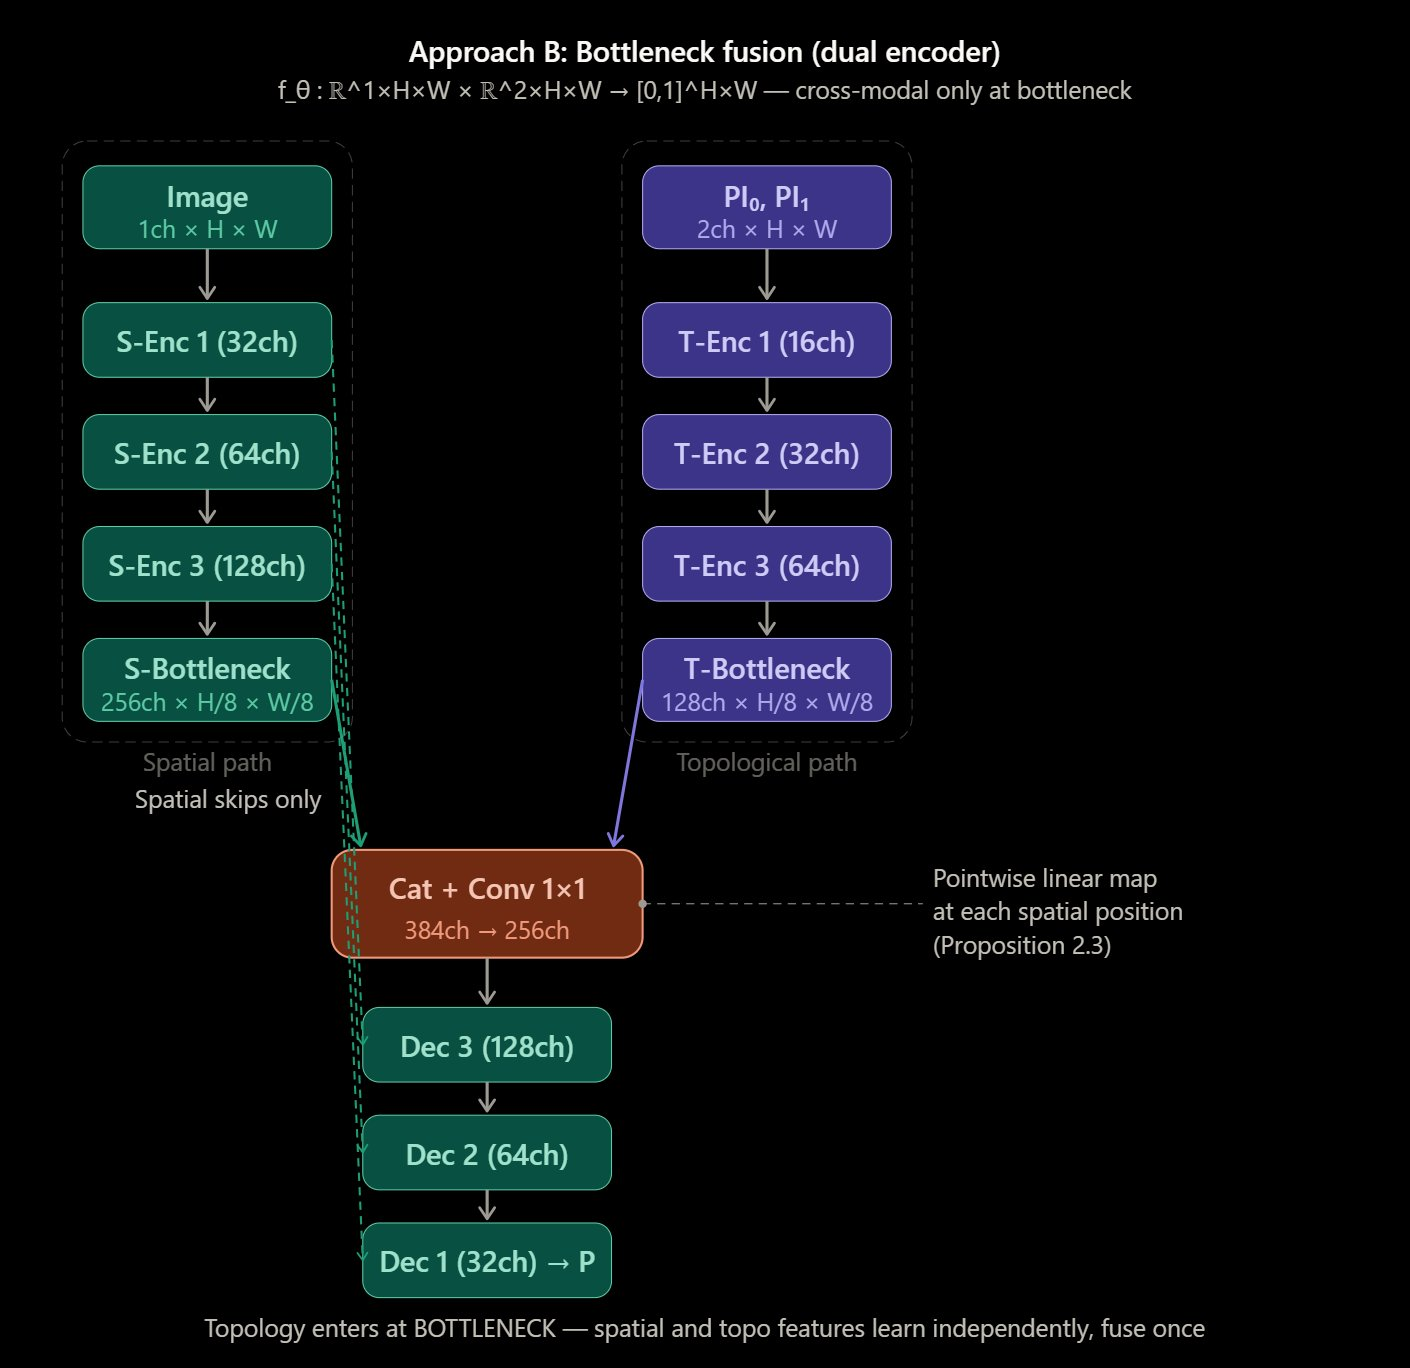
\includegraphics[width=\columnwidth]{arch_bottleneck.png}
\caption{BottleneckFusion: encoders espacial (izq.) y topológico (der.) independientes. Fusión solo en el bottleneck via Cat + Conv$_{1\times1}$.}
\label{fig:bottleneck}
\end{figure}

% ============================================================
\section{Pipeline TDA}

Para cada muestra, la extracción topológica procede como:
\begin{enumerate}[noitemsep]
\item Máscara binaria $M \to \text{EDT}(M)$ (transformada de distancia euclidiana)
\item $-\text{EDT}(M) \to$ Complejo cubical $\to$ Homología persistente
\item Diagramas $\text{Dgm}_0, \text{Dgm}_1 \to$ Imágenes de persistencia $\text{PI}_0, \text{PI}_1$
\end{enumerate}

Parámetros: bandwidth $\sigma = 1.0$, filtración máxima $= 30.0$, resolución PI $= 20 \times 20$ (upsampled a $128 \times 128$).

Durante entrenamiento: PI se computan sobre la verdad (GT). Durante evaluación: inferencia de dos pasadas.

% ============================================================
\section{Funciones de Pérdida}

\subsection{SoftDiceLoss}
\begin{equation}
\mathcal{L}_{\text{Dice}} = 1 - \frac{2 \sum P \cdot M + \varepsilon}{\sum P + \sum M + \varepsilon}, \quad \varepsilon = 10^{-5}
\end{equation}

\subsection{BettiMatchingLoss \cite{stucki2023}}

Dada la predicción $P$ y la verdad $G$, se construye $C = \max(P, G)$. Las inclusiones $P \hookrightarrow C$ y $G \hookrightarrow C$ inducen matchings en homología persistente:
\begin{equation}
\mathcal{L}_{\text{BM}} = \sum_{\text{no emparejados}} (d_i - b_i)^2
\end{equation}

\subsection{Entrenamiento Curricular}

\begin{itemize}[noitemsep]
\item \textbf{Warmup} (ép. 1--15): $\mathcal{L} = \mathcal{L}_{\text{Dice}}$
\item \textbf{Rampa} (ép. 16--36): $\lambda: 0 \to 0.3$
\item \textbf{Completo} (ép. 37--60): $\lambda = 0.3$
\end{itemize}

Tres modos: \texttt{dice} ($\mathcal{L}_{\text{Dice}}$ siempre), \texttt{betti} ($\mathcal{L}_{\text{BM}}$ puro tras warmup), \texttt{dice+betti} ($(1-\lambda)\mathcal{L}_{\text{Dice}} + \lambda\mathcal{L}_{\text{BM}}$).

% ============================================================
\section{Configuración Experimental}

Dataset: 500 train / 200 test, resolución $128\times128$, 60 épocas, Adam ($\text{lr}=10^{-3}$, weight decay $10^{-5}$), CosineAnnealingLR, batch size 8, seed 42. Dispositivo: TPU v5e-1 para Baseline\_dice; CPU para el resto.

Dataset con 4 niveles de dificultad topológica: fácil (15\%), medio (30\%), difícil (35\%), extremo (20\%). Formas: discos, donuts, donuts ultra-finos (2px pared), discos tocándose (1px gap), anillos anidados, anillos rotos.

% ============================================================
\section{Resultados}

\subsection{Tabla Completa}

\begin{table}[H]
\centering
\caption{Resultados de los 12 experimentos (9 originales + 3 corregidos). $\star$ indica cero errores.}
\label{tab:results}
\resizebox{\columnwidth}{!}{
\begin{tabular}{llcccc}
\toprule
\textbf{Arquitectura} & \textbf{Pérdida} & \textbf{Dice}$\uparrow$ & $\beta_0$\textbf{Err}$\downarrow$ & $\beta_1$\textbf{Err}$\downarrow$ & \textbf{Min} \\
\midrule
Baseline & dice & \textbf{0.9772} & 0.180 & 0.260 & 2.7 \\
Baseline & betti (corr.) & 0.9697 & \textbf{0.100} & 0.040 & 122.7 \\
Baseline & dice+betti & 0.9763 & 0.105 & 0.040 & 162.8 \\
\midrule
InputFusion & dice & \textbf{0.9789} & 0.150 & 0.040 & 153.5 \\
InputFusion & betti (corr.) & 0.9660 & \textbf{0.100} & 0.020 & 115.7 \\
InputFusion & dice+betti & 0.9764 & 0.110 & 0.010 & 184.9 \\
\midrule
BotFusion$^*$ & dice & 0.9774 & 0.180 & 0.075 & 197.0 \\
BotFusion$^*$ & betti (corr.) & 0.9684 & 0.105 & \textbf{0.005} & 130.8 \\
BotFusion$^*$ & dice+betti & 0.9766 & 0.115 & $\mathbf{0.000}^\star$ & 186.6 \\
\bottomrule
\end{tabular}
}
\smallskip
\footnotesize{$^*$Propuesta nuestra. (corr.) = modo betti-only corregido.}
\end{table}

\subsection{Resultados Estratificados}

\begin{table}[H]
\centering
\caption{BottleneckFusion dice+betti por dificultad.}
\label{tab:stratified}
\begin{tabular}{lcccc}
\toprule
\textbf{Nivel} & \textbf{n} & \textbf{Dice} & $\beta_0$ & $\beta_1$ \\
\midrule
Fácil & 36 & 0.9988 & 0.000 & 0.000 \\
Medio & 65 & 0.9861 & 0.000 & 0.000 \\
Difícil & 61 & 0.9759 & 0.377 & 0.000 \\
Extremo & 38 & 0.9407 & 0.000 & 0.000 \\
\midrule
\textbf{Total} & \textbf{200} & \textbf{0.9766} & \textbf{0.115} & $\mathbf{0.000}$ \\
\bottomrule
\end{tabular}
\end{table}

\subsection{Componentes de Pérdida}

\begin{table}[H]
\centering
\caption{Componentes de pérdida — BotFusion betti-only (corregido).}
\label{tab:components}
\begin{tabular}{cccccc}
\toprule
\textbf{Ép.} & \textbf{Loss} & \textbf{Dice} & \textbf{BM} & \textbf{Ratio} & \textbf{Modo} \\
\midrule
1 & 0.618 & 0.618 & 0.000 & 0.00 & Warmup \\
10 & 0.049 & 0.049 & 0.000 & 0.00 & Warmup \\
20 & 0.147 & 0.117 & 0.147 & 1.26 & BM only \\
40 & 0.034 & 0.043 & 0.034 & 0.77 & BM only \\
60 & 0.027 & 0.039 & 0.027 & 0.69 & BM only \\
\bottomrule
\end{tabular}
\end{table}

La ratio BM/Dice se estabiliza en 0.69--0.77, confirmando que ambas pérdidas operan en escalas comparables.

% ============================================================
\section{Análisis y Discusión}

\subsection{Hallazgo 1: Betti Matching reduce errores drásticamente}

Comparando modo dice vs.\ dice+betti:
\begin{itemize}[noitemsep]
\item Baseline: $\beta_1$ baja de 0.260 a 0.040 ($-85\%$)
\item InputFusion: $\beta_1$ baja de 0.040 a 0.010 ($-75\%$)
\item BottleneckFusion: $\beta_1$ baja de 0.075 a 0.000 ($-100\%$)
\end{itemize}
El Dice se mantiene esencialmente constante (caída máxima de 0.0008).

\subsection{Hallazgo 2: BottleneckFusion supera a InputFusion}

\begin{table}[H]
\centering
\caption{Comparación directa en modo dice+betti.}
\label{tab:headtohead}
\begin{tabular}{lccc}
\toprule
\textbf{Métrica} & \textbf{InputFusion} & \textbf{BotFusion} & \textbf{Ganador} \\
\midrule
Dice & 0.9764 & \textbf{0.9766} & Nuestro \\
$\beta_0$ Err & \textbf{0.110} & 0.115 & Paper \\
$\beta_1$ Err & 0.010 & $\mathbf{0.000}$ & \textbf{Nuestro} $\star$ \\
\bottomrule
\end{tabular}
\end{table}

\subsection{Hallazgo 3: Las PI son informativas por sí solas}

InputFusion\_dice (sin pérdida topológica) logra $\beta_1 = 0.040$, comparado con Baseline\_dice $\beta_1 = 0.260$ --- una reducción del 85\%.

\subsection{Hallazgo 4: El modo betti-only revela el trade-off}

El modo betti-only sacrifica $\sim$0.8--1.3\% de Dice pero logra los mejores $\beta_0$ (0.100). La mezcla dice+betti es el óptimo de Pareto.

\subsection{Principio de Separación de Gradientes}

\begin{proposition}[Conflicto de gradientes en InputFusion]
Sea $p_c$ un píxel crítico que es falso positivo ($P(p_c) > 0.5$, $G(p_c) = 0$) pero topológicamente necesario (cierra un gap que restaura $\beta_1$). Entonces para cualquier parámetro compartido $w$:
\begin{equation}
\text{sign}\left(\frac{\partial \mathcal{L}_{\text{Dice}}}{\partial w}\right) = -\text{sign}\left(\frac{\partial \mathcal{L}_{\text{BM}}}{\partial w}\right)
\end{equation}
Los gradientes apuntan en direcciones opuestas.
\end{proposition}

En BottleneckFusion, con $\theta_{\text{spatial}} \cap \theta_{\text{topo}} = \emptyset$, este conflicto se resuelve arquitectónicamente: cada encoder recibe gradientes que no interfieren con el otro.

\subsection{Corrección del Bug}

Los experimentos originales tenían un bug: los modos ``betti'' y ``dice+betti'' usaban la misma fórmula. La corrección implementó un verdadero modo betti-only: $\mathcal{L} = \mathcal{L}_{\text{BM}}$ sin componente Dice después del warmup.

% ============================================================
\section{Limitaciones}

\begin{enumerate}[noitemsep]
\item Datos sintéticos --- validación en BraTS pendiente
\item Un solo seed --- sin pruebas de significancia estadística
\item Sin validación cruzada
\item Dispositivo heterogéneo (TPU vs.\ CPU)
\item Pipeline TDA no diferenciable
\end{enumerate}

% ============================================================
\section{Conclusiones}

\begin{enumerate}[noitemsep]
\item La pérdida de Betti Matching reduce errores topológicos 75--100\% sin sacrificar Dice.
\item BottleneckFusion alcanza \textbf{cero errores $\beta_1$} bajo supervisión topológica.
\item El \emph{Principio de Separación de Gradientes} ($\theta_{\text{spatial}} \cap \theta_{\text{topo}} = \emptyset$) explica esta superioridad.
\item Las imágenes de persistencia reducen $\beta_1$ un 85\% incluso sin pérdida topológica.
\item La mezcla dice+betti con curriculum es el óptimo de Pareto.
\end{enumerate}

% ============================================================
\section{Próximos Pasos}

\begin{enumerate}[noitemsep]
\item Validar en BraTS 2023 Meningioma
\item Implementar baselines DG (Chan-Vese, contornos activos geodésicos)
\item Implementar pérdidas DG+NN (Mumford-Shah, regresión EDT)
\item Tabla comparativa de 4 cuadrantes (AT$\pm$NN, DG$\pm$NN)
\end{enumerate}

% ============================================================
\begin{thebibliography}{9}
\bibitem{stucki2023} Stucki, N., Paetzold, J.C., Shit, S., Menze, B., Bauer, U. (2023). Topologically Faithful Image Segmentation via Induced Matching of Persistence Barcodes. \emph{ICML}.
\bibitem{ronneberger2015} Ronneberger, O., Fischer, P., Brox, T. (2015). U-Net: Convolutional Networks for Biomedical Image Segmentation. \emph{MICCAI}.
\bibitem{adams2017} Adams, H. et al. (2017). Persistence Images: A Stable Vector Representation. \emph{JMLR}, 18(8), 1--35.
\bibitem{yu2020} Yu, T. et al. (2020). Gradient Surgery for Multi-Task Learning. \emph{NeurIPS}.
\bibitem{berger2025} Berger, C. et al. (2025). Pitfalls of Topology-Aware Image Segmentation. \emph{IPMI}.
\bibitem{cohen2007} Cohen-Steiner, D., Edelsbrunner, H., Harer, J. (2007). Stability of Persistence Diagrams. \emph{DCG}, 37(1), 103--120.
\bibitem{etmann2023} Etmann, C. et al. (2023). A Unified Framework for U-Net Design and Analysis. arXiv:2305.19638.
\end{thebibliography}

\end{document}